\documentclass[11.5pt, paper=a4]{article}

\usepackage[utf8]{inputenc}
\usepackage[english]{babel}
\usepackage[T1]{fontenc}

\usepackage{amsmath, amssymb, amscd, amsthm, amsfonts, mathtools}
\usepackage[left=2cm, right=2cm, top=1.5cm]{geometry}

\usepackage{graphicx}
\usepackage{graphicx}
\usepackage{hyperref}
\usepackage{physics}
\usepackage{tikz}
\usepackage{url}
\usepackage[square,numbers]{natbib} \usepackage{tabularx}
\usetikzlibrary{quantikz}

\usepackage{braket}
\usepackage{thmtools}
\usepackage{float}

%%% Theorem Style
\theoremstyle{definition}
\newtheorem{theorem}{Theorem}[section]
\newtheorem{definition}[theorem]{Definition}
\newtheorem{lemma}[theorem]{Lemma}
\newtheorem{conjecture}[theorem]{Conjecture}
\newtheorem{corollary}[theorem]{Corollary}

\numberwithin{theorem}{section}

%% Autoref prefixes
\renewcommand{\sectionautorefname}{Section}
\renewcommand{\subsectionautorefname}{Section}
\renewcommand{\subsubsectionautorefname}{Section}
\renewcommand{\figureautorefname}{Figure}
\def\theoremautorefname{Theorem}
\def\lemmaautorefname{Lemma}
\def\definitionautorefname{Definition}
\def\conjectureautorefname{Conjecture}
\def\algorithmautorefname{Algorithm}

%% Writing algorithms

\usepackage{algorithm} % captioning 
\usepackage{algpseudocode}
\usepackage{braket}
\usepackage{physics}
\usepackage{mathtools}
\usepackage{amsmath}
\usepackage[utf8]{inputenc}
\usepackage{ulem}
% \def\NoNumber#1{{\def\alglinenumber##1{}\State #1}\addtocounter{ALG@line}{-1}}

\usepackage{tikz}

% TikZ libraries `calc` needed now to tweak bracket.
\usetikzlibrary{backgrounds,fit,decorations.pathreplacing,calc}
% Dirac Kets
\newcommand{\ket}[1]{\ensuremath{\left|#1\right\rangle}}

\title{Quantum Algorithms, Spring 2022: Lecture 18 Scribe}

\author{Hrishi Narayanan and Sabyasachi Mukhopadhay}

\date{\today}

\begin{document}

\maketitle

\section{Unstructured Search Problem}
Given the set of $N$ elements, $X = \{X_1,\ldots, X_N\}$ and a given boolean function $f:X\to \{0, 1\}$, the goal is to find an element $x^* \in X$ such that $f(x^*) = 1$. Here, $N = 2^n$. Also, let $M \ll N$ be the number of elements $\{x_i\}$ in $X$ such that $f(x_i) = 1$.

\subsection{Problem Statement}
Given a black box $U_f$ for the boolean function $f$, how many queries are needed to find $x^*$ such that $f(x^*) = 1$?

\begin{itemize}
    \item \uline{Classical}: Classically, this can be done in $O(N/M)$ queries.
    \item \uline{Quantum}: We solve this problem using Grover’s search algorithm.
\end{itemize}

\section{Grover's Search}
\begin{center}
\begin{quantikz}
\lstick{$\ket 0 ^ {\otimes n}$} & \gate[wires=1]{H^{\otimes n}} & \gate{U_f^{\pm}} & \gate{D} & \qw\ \ldots\ & \gate{U_f^{\pm}} & \gate{D} & \meter{} & \cw \\
\end{quantikz}
\end{center}

Here, $G = DU_f^{\pm}$ is applied repeatedly. Now, let $H^{\otimes n} \ket{0}^{\otimes n} = \frac{1}{\sqrt N} \sum_{x \in {0, 1}^n} \ket{x} = \ket{s}$. Now, we have $\ket{s} = \sqrt{\frac{M}{N}} \ket{w} + \sqrt{\frac{N - M}{N}} \ket{s_{\Bar{w}}} = \sin(\frac{\theta}{2})\ket{w} + \cos(\frac{\theta}{2})\ket{s_{\Bar{w}}}$, where $\ket{w}$ and $\ket{s_{\Bar{w}}}$ are described as follows.

$$\ket{w} = \sqrt{\frac{1}{M}} \sum_{x: f(x) = 1} \ket{x}$$
$$\ket{s_{\Bar{w}}} = \sqrt{\frac{1}{N - M}} \sum_{x: f(x) = 0} \ket{x}$$

\subsection{Oracle}
$$U_f^{\pm}\ket{w} = - \ket{w}$$
$$U_f^{\pm}\ket{s_{\Bar{w}}} = \ket{s_{\Bar{w}}}$$

In the $2-$D subspace spanned by $\{\ket{s_{\Bar{w}}}, \ket{w}\}$, we have $U_f^{\pm} = \begin{bmatrix}1 & 0\\ 0 & -1\end{bmatrix} = \mathbb{I} - 2\ket{w}\bra{w}$.

\subsection{Diffuser}
Here, $V_0$ represents conditional phase flip which flips phase of all computational basis states other than $0^n$. For any quantum state $\ket{\phi} = \sum_k \alpha_k \ket{k}$, $D\ket{\phi} = \sum_k (2\left<\alpha\right> - \alpha_k)\ket{k}$ which performs inversion about the mean.

$$V_0 = 2 \ket{0^n}\bra{0^n} - \mathbb{I}$$
$$\implies D = H^{\otimes n} V_0 H^{\otimes n} = 2 \ket{s}\bra{s} - \mathbb{I}$$

\begin{figure}[H]
    \centering
    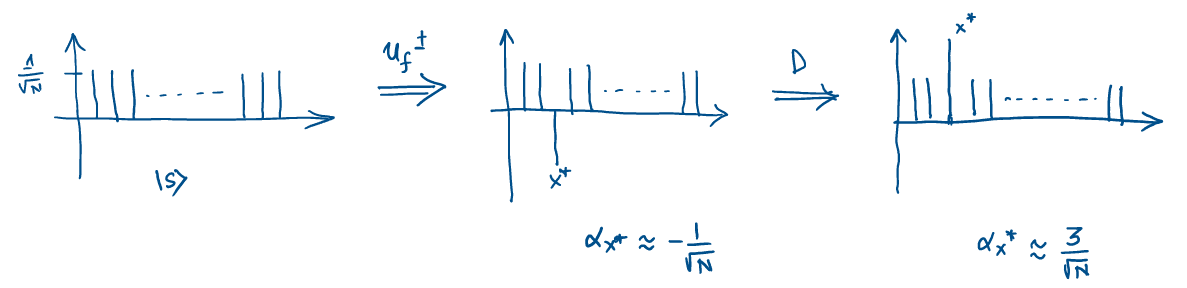
\includegraphics[width=100mm]{images/1.png}
    % \caption{Caption}
    % \label{fig:my_label}
\end{figure}

In the $2-$D subspace spanned by $\{\ket{s_{\Bar{w}}}, \ket{w}\}$ we have, $D = 2\ket{s}\bra{s} - \mathbb{I}$ is as follows.

$$D = \begin{bmatrix}\cos \theta & \sin \theta\\ \sin \theta & -\cos \theta\end{bmatrix}$$

\section{Grover Iterate}
$$G = DU_f^{\pm}$$

As $D = 2\ket{s}\bra{s} - \mathbb{I}$ and $U_f^{\pm} = \mathbb{I} - 2 \ket{w}\bra{w}$, $G = - R_s R_w$ is a product of two two reflections which is equivalent to a rotation. $G$ induces a rotation by an angle $\theta$ in the $2-$D subspace spanned by $\{\ket{s_{\Bar{w}}}, \ket{w}\}$. $G$ rotates $\ket{s}$ gradually towards $\ket{w}$.

$$G = \begin{bmatrix}\cos \theta & \sin \theta\\ \sin \theta & -\cos \theta\end{bmatrix}\begin{bmatrix}1 & 0\\ 0 & -1 \end{bmatrix} = \begin{bmatrix}\cos \theta & -\sin \theta\\ \sin \theta & \cos \theta\end{bmatrix}$$

\begin{figure}[H]
    \centering
    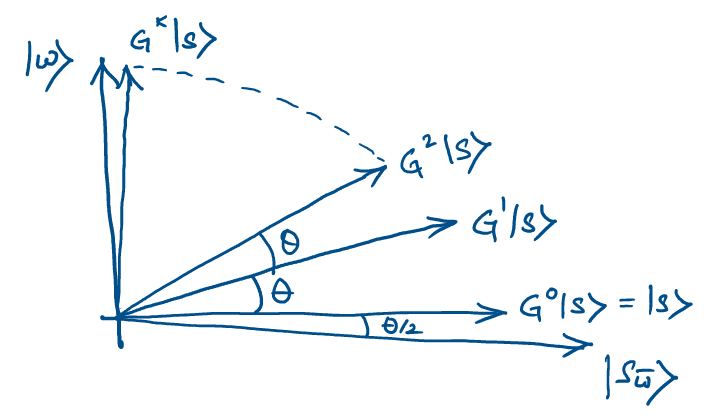
\includegraphics[width=80mm]{images/2.png}
    % \caption{Caption}
    % \label{fig:my_label}
\end{figure}

$$\ket{s} = \cos \frac{\theta}{2} \ket{s_{\Bar{w}}} + \sin \frac{\theta}{2} \ket{w}$$

\subsection{Finding optimal $k$}
We are required to find $k$ such that $|\bra{w}G^k\ket{s}|^2 \approx 1$.

$$G = \begin{bmatrix}\cos \theta & -\sin \theta\\ \sin \theta & \cos \theta\end{bmatrix}\ \text{ and }\ \ket{s} = \begin{bmatrix}\cos \frac{\theta}{2}\\ \sin \frac{\theta}{2}\end{bmatrix}$$

$$\implies G^k\ket{s} = \sin\frac{(2k + 1)\theta}{2} \ket{w} + \cos \frac{(2k + 1)\theta}{2}\ket{s_{\Bar{w}}}$$

Now, $\sin \frac{\theta}{2} = \sqrt{\frac{M}{N}}$ and for $|\bra{w}G^k\ket{s}|^2 \approx 1$ we must have $\sin \frac{(2k + 1)\theta}{2} \approx 1 \implies \frac{(2k + 1)\theta}{2} = \frac{\pi}{2} \implies \theta = \frac{\pi}{2k + 1}$.

$$\implies 2 \sin^{-1} \sqrt{\frac{M}{N}} = \frac{\pi}{2k + 1}$$

And, since $M \ll N$, we have $\sin \frac{\theta}{2} \approx \frac{\theta}{2}$ $\implies 2 \sqrt{\frac{M}{N}} = \frac{\pi}{2k + 1} \implies 2k + 1 = \frac{\pi}{2}\sqrt{\frac{N}{M}}$. Thus, $k_{\text{opt}} = \lceil{\frac{\pi}{4}\sqrt{\frac{N}{M}} - \frac{1}{2}}\rceil$. \newline

After these many iterations, we end up with a state close to $\ket{w}$ such that $\ket{w} = \frac{1}{\sqrt M} \sum_{x: f(x) = 1} \ket{x}$. By making a measurement in the computational basis, we observe some $x^*: f(x^*) = 1$.

\begin{figure}[H]
    \centering
    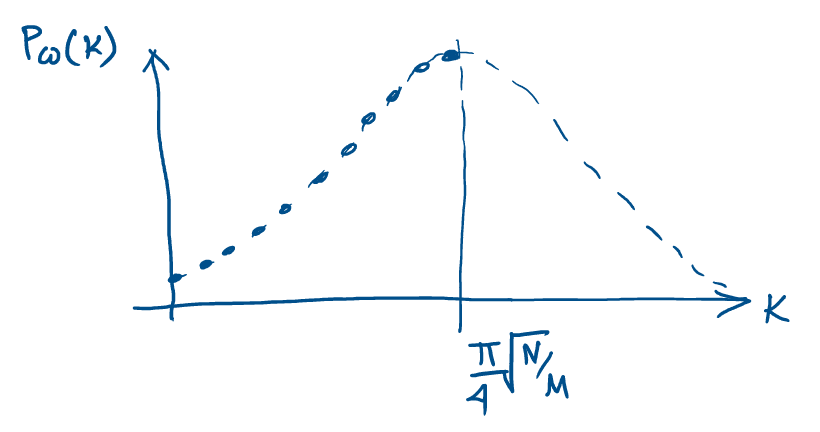
\includegraphics[width=70mm]{images/3.png}
    % \caption{Caption}
    % \label{fig:my_label}
\end{figure}

As evident from the above figure, we have overshooting problems with $k$. But, there are ways to get around.

\begin{itemize}
    \item Randomized Quantum Search: $O(\sqrt N)$ iterations, one can obtain $x^*$ with $\Theta{(1)}$ probability.
    \item Quantum Counting: Use QPE on the Grover iterate $G$ to estimate $M$ to some accuracy.
\end{itemize}

\section{Randomized Quantum Search}
\begin{enumerate}
    \item Set $K = 0$.
    \item Set $M = 2^k$.
    \item Run Grover's algorithm for $\frac{\pi}{4}\sqrt{\frac{N}{M}}$ iterations.
    \item If a solution is found then EXIT. Otherwise, go to step 5.
    \item $K = K + 1$.
    \item If $K > \log_2 N$, then EXIT. Otherwise, go to step 2.
\end{enumerate}

We run Grover's algorithm using $M = 1$, if it fails, try again with $M = 2, 4, 8, \ldots, 2^{\log_2 N}$.

\subsection{Query Complexity}
Total number of queries in the worst case $= \sum_{l = 0}^{\log_2 N} \frac{\pi}{4} \sqrt{\frac{N}{2^l}} = \frac{\pi}{4}\sqrt{N} \sum_{l = 0}^{\log_2 N} \left(\frac{1}{\sqrt 2}\right)^l = O(\sqrt N)$. There will be a guess $M$ such that $M'/2 \leq M \leq 2M'$. And, there $\exists\ j$, such that $\frac{p}{2} \leq 2^j \leq 2p$ for $p \in \mathbb{N}\ \equiv\ \exists$ a positive integer between $\log_2 p - 1$ and $\log_2 p + 1$. \newline

For $M$ such that $\frac{M'}{2} \leq M \leq 2M'$, the Grover's algorithm is run for $T = \frac{\pi}{4}\sqrt{\frac{N}{M}}$ iterations. This also means that $T$ is within a factor of $\sqrt{2}$ of $T' = \frac{\pi}{4}\sqrt{\frac{N}{M'}}$, the optimal number of iterations. Thus, we have $(2T' + 1) \sin^{-1}\left(\sqrt{\frac{M'}{N}}\right) = \frac{\pi}{2}$.

\subsection{Success Probability}
$$\sin^2\left((2T + 1) \sin^{-1} \left(\sqrt{\frac{M'}{N}}\right) \right) = \sin^2\left(\frac{2T + 1}{2T' + 1} \frac{\pi}{2}\right) \approx \sin^2 \left(\frac{T}{T'}\frac{\pi}{2}\right) = \sin^2 \left(\sqrt{\frac{M'}{M}}\frac{\pi}{2}\right) = \sin^2 \left(\delta \frac{\pi}{2}\right) = \Theta{(1)}$$

\begin{itemize}
    \item Here, $\frac{1}{\sqrt 2} \leq \delta \leq \sqrt 2$.\newline
    \item Randomized quantum search finds $x^*$ with constant probability in $O(\sqrt N)$ queries even when $M$ is unknown.
    \item When $M$ is very close to $N$ ($M < N / 2$), $|\left<w | s\right>|^2 \geq 1/2$.So just preparing $\ket{s}$ followed by measurements would suffice.
    \item If $M = 0$, use quantum computing to estimate $M$.
\end{itemize}

\nocite{*}
\bibliographystyle{plainnat}
\bibliography{references}
\end{document}